\documentclass{math201}
\usepackage{hyperref}
\usepackage{bookmark}
\usepackage{minted}

% =============================================
% Part 0 信息
% =============================================

\mathsetup{
  % 学生姓名
  student = {某同学},
  % 学号
  student-id = {2021xxxx},
  % 院系
  experiment = {实验7 RTC-闹钟实验 + LCD 实验},
  % 专业年级
  discipline = {集成电路设计与集成系统},
  % 日期
  date = {\today},
}

\begin{document}

% =============================================
% Part 1  封面
% =============================================

\makecover

% =============================================
% Part 2 主文档
% =============================================

\section{实验要求}

\begin{enumerate}
  \item 运行例程实验8 RTC—日历实验、实验13RTC—闹钟实验+LCD实验 ,观察实验现象
  \item 看懂源程序
  \item 修改源程序,实现时间显示修改源程序时的日期与时间,分别通过LCD和串口显示日期和时间,并利用闹钟中断设定一个闹钟,闹钟时间到时蜂鸣器响。 (源程序中不需要的内容全部删掉)
  \item 撰写实验报告,把修改的程序截图、实验现象的截图或者图片整理到报告中。
\end{enumerate}

\section{实验内容及结果}

\subsection{编写代码}

需要修改 \texttt{bsp\_rtc.h} 文件。

\begin{minted}[
  frame=lines,
  framesep=2mm,
  baselinestretch=1.2,
  fontsize=\small,
]{C++}
// 时间宏定义
#define RTC_H12_AMorPM            RTC_H12_AM  
#define HOURS                     8          // 0~23
#define MINUTES                   50          // 0~59
#define SECONDS                   1          // 0~59


// 日期宏定义
#define WEEKDAY                   3         // 1~7
#define DATE                      10         // 1~31
#define MONTH                     4         // 1~12
#define YEAR                      24        // 0~99

// 闹钟相关宏定义
#define ALARM_HOURS               8          // 0~23
#define ALARM_MINUTES             50         // 0~59
#define ALARM_SECONDS             15          // 0~59
\end{minted}

为了避免闹钟一直响,可以修改 \texttt{stm32f4xx\_it.c} 文件中的 \texttt{ RTC\_Alarm\_IRQHandler} 函数,添加关闭蜂鸣器的代码。

\begin{minted}[
  frame=lines,
  framesep=2mm,
  baselinestretch=1.2,
  fontsize=\small,
]{C++}
// 闹钟中断服务函数
void RTC_Alarm_IRQHandler(void)
{
  if (RTC_GetITStatus(RTC_IT_ALRA) != RESET)
  {
    RTC_ClearITPendingBit(RTC_IT_ALRA);
    EXTI_ClearITPendingBit(EXTI_Line17);
  }
  /* 闹钟时间到,蜂鸣器响 */
  BEEP_ON;
  Delay(0x5fffff);
  BEEP_OFF;
}

void Delay(__IO uint32_t nCount) // 简单的延时函数
{
  for (; nCount != 0; nCount--)
    ;
}
\end{minted}

\subsection{下载运行}

使用 \texttt{FlyMCU.exe} 下载程序到 STM32 开发版上,观察实验现象。

\subsection{实验现象}

\begin{figure}[H]
  \centering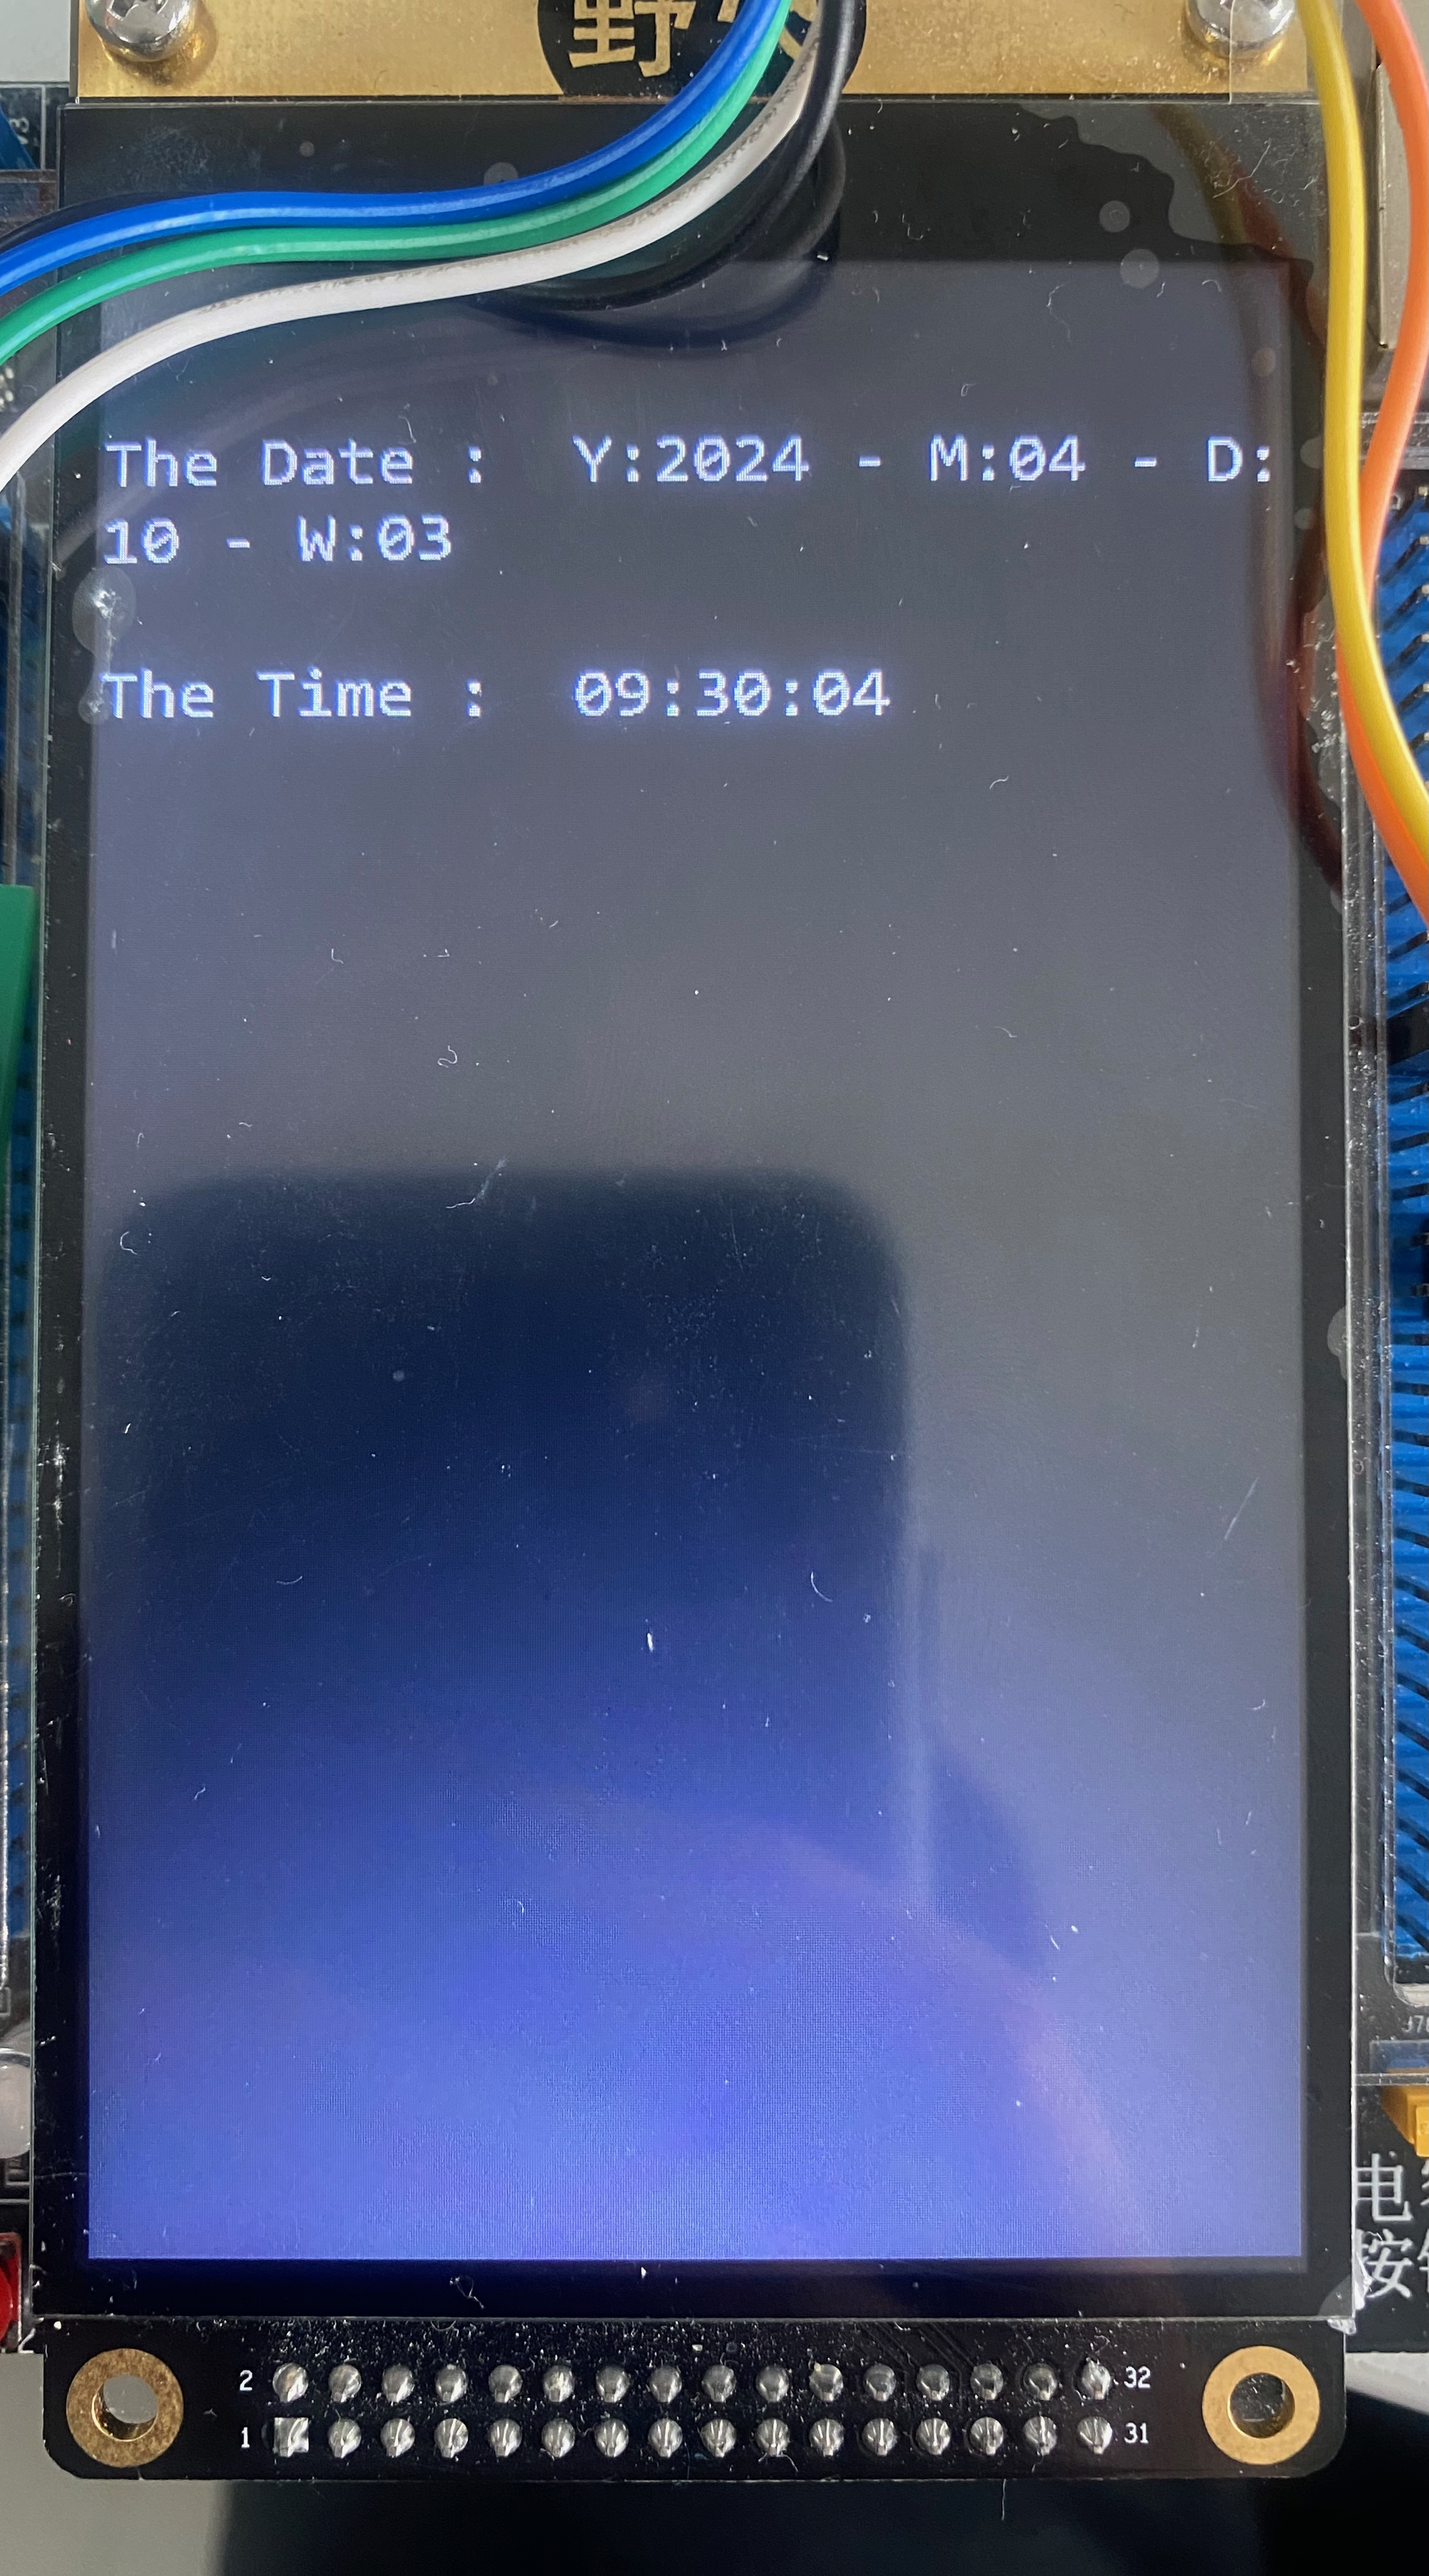
\includegraphics[width=0.6\linewidth]{rtc_show_time.jpeg}
  \caption{RTC 显示时间}
\end{figure}

\section{实验小结}

通过本次实验,学会了如何使用 RTC 实时时钟模块,实现时间的显示和闹钟功能。

\end{document}
